\documentclass[a4paper, 12pt]{article}
\usepackage[a4paper, top = 1.5cm, bottom = 1.5cm, left = 1cm, right = 1cm]{geometry}
\usepackage{graphicx}
\usepackage{subcaption}
\usepackage{mathtools}
\usepackage{amsfonts}
\usepackage[english, russian]{babel}
\title{Лабораторная работа № 3.1.3 "Измерение магнитного поля Земли"}
\author{Кирилл Шевцов Б03-402}
\date{8.09.2025}
\begin{document}
\maketitle
\section*{Цель работы}
Исследовать свойства постоянных неодимовых магнитов, с их помощью измерить горизональную и вертикальную составляющую индукции магнитного поля Земли и наклонение.
\section*{Оборудование}
Неодимовые магниты, тонкая нить для изготовления крутильного маятника, медная проволока, электронные весы, секундомер, измеритель магнитной индукции, штангенциркуль.
\section*{Экспериментальная установка}
Следующие установки помогут измерить: период крутильных колебаний (\ref{sub@крутильный маятник}), силу отрыва цепочки шариков (\ref{sub@установка для силы отрыва}),
магнитный момент для двух шариков (\ref{sub@магнитный момент установка}).
\begin{figure}[htbp]
        \centering
        \begin{subfigure}{0.2\textwidth}
            \centering
            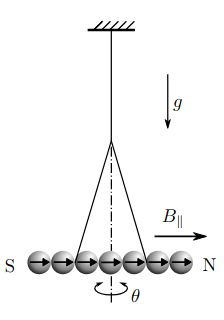
\includegraphics[width=\linewidth]{p1.png}
            \caption{крутильный маятник}
            \label{крутильный маятник}
        \end{subfigure}
        \hspace{2cm}
        \begin{subfigure}{0.2\textwidth}
            \centering
            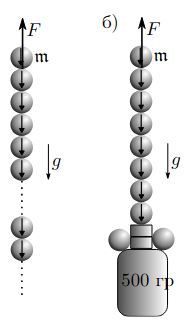
\includegraphics[width=\linewidth]{p2.png}
            \caption{установка для силы отрыва}
            \label{установка для силы отрыва}
        \end{subfigure}
        \hspace{2cm}
        \begin{subfigure}{0.2\textwidth}
            \centering
            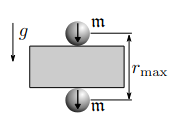
\includegraphics[width=\linewidth]{p3.png}
            \caption{измерение магнитного момента}
            \label{магнитный момент установка}
        \end{subfigure}
        \caption{экспериментальные установки}
        \label{установки}
    \end{figure}\\
Две последние установки дают один результат для измерения магнитного момента. Можно скрутить магнитную стрелку в кольцо, и
показать, что упругость нити при вычислении периода колебаний стрелки можно не учитывать.
\begin{figure}[htbp]
    \centering
    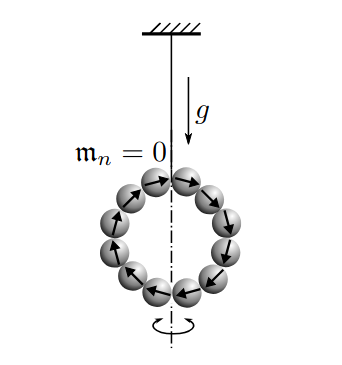
\includegraphics[width=0.3\linewidth]{p4.png}
    \caption{магнитная стрелка, свернутая в кольцо}
    \label{магнитная стрелка, свернутая в кольцо}
\end{figure}
\section*{Необходимые формулы и теория}
\paragraph{}
Простейший магнитный диполь может быть образован витком с током или постоянным магнитом.\\
Магнитное поле точечного диполя вычисляется подобно формуле напряженности электрического поля этого диполя:
\begin{equation}
    \mathbf{B} = \frac{\mu_{0}}{4 \pi}\left(\frac{3({\mathfrak{m}} \cdot \mathbf{r}) \mathbf{r}}{r^{5}} - \frac{{\mathfrak{m}}}{r^{3}}\right)
    \label{Магнитное поле диполя}
\end{equation}
Здесь $\mu_{0} = 4\pi \cdot 10^{-7}$ Гн/м - магнитная постоянная, $\mathbf{\mathfrak{m}}$ - магнитный момент точечного диполя, $\mathbf{r}$ - радиус вектор, направленный от диполя в рассматриваемую точку.\\
Во внешнем магнитном поле с индукцией $\mathbf{B}$ на точечный магнитный диполь $\mathfrak{m}$ действует механический момент сил:
\begin{equation}
    \mathbf{M} = [\mathfrak{m} \times \mathbf{B}]
    \label{Момент}
\end{equation}
В неоднородном магнитном поле на точечный диполь действует сила:
\begin{equation}
    \mathbf{F} = (\mathfrak{m} \cdot \nabla)\mathbf{B}
    \label{Сила действия на диполь}
\end{equation}
В частности, проекция силы на ось $\mathit{Ox}$:
\begin{equation}
    F_{x} = \mathfrak{m}_{x}\frac{\partial B_{x}}{\partial x} + \mathfrak{m}_{y}\frac{\partial B_{x}}{\partial y} + \mathfrak{m}_{z}\frac{\partial B_{x}}{\partial z}
    \label{Проекция силы}
\end{equation}
\paragraph{}
Формулы (\ref{Момент}) и (\ref{Сила действия на диполь}) помогают рассчитать силу взаимодействия магнитов с моментами $\mathfrak{m_{1}}$ и $\mathfrak{m_{2}}$ в рамках точечных диполей:
\begin{equation}
    F_{12} = \mathfrak{m}_{1}{\frac{\partial {B_{2}}}{\partial r}} = \mathfrak{m}_{1}\frac{\partial (2\mathfrak{m}_{2}/r^{3})}{\partial r}  =-6\frac{\mathfrak{m}_{1}\mathfrak{m}_{2}}{r^{4}}
    \label{Сила взаимодействия диполей}
\end{equation}
Для рассчета магнитного поля Земли есть несколько методов:
\begin{enumerate}
    \item Определить магнитный момент $\mathfrak{m}$ двух из шариков, определив наибольшее расстояние $\mathit{r_{max}}$, на котором они смогут удерживать друг друга в поле тяжести. По величине $\mathfrak{m}$\
    с помощью (\ref{Магнитное поле диполя}) рассчитать величину индукции вблизи любой точки на поверхности шара радиусом $\mathit{R}$.
    \begin{equation}
        \mathfrak{m} = \sqrt{\frac{mgr_{max}^{4}}{6}}
        \label{Магнитный момент}
    \end{equation}
    Учтем, что здесь магнитный момент представлен вычислением в единицах СГС.
    \item Величину магнитного поля можно определить с помощью силы сцепления намагниченных шариков. Определим ее, как необходимую силу для разрыва двух сцепившихся шариков. Сила сцепления (\ref{Сила взаимодействия диполей}) равна:
    \begin{equation}
        F_{0} = \frac{6\mathfrak{m}^{2}}{(2R)^{4}} = \frac{3\mathfrak{m}^2}{8R^{4}}
        \label{Сила сцепления}
    \end{equation}
    Минимальный вес цепочки, при которой она оторвется от верхнего шарика, равна:
    \begin{equation}
        F = F_{0}\left(\sum_{k = 1}^n \frac{1}{k^{4}}\right) \approx 1,08F_{0}
        \label{Вес цепочки}
    \end{equation}
    Учтём, что сила сцепления шариков при их отрывании убывает как $1/r^{4}$.
    \item Рассчитать магнитное поле Земли можно с помощью составляющих: вертикальной и горизонтальной, ведь:
    \begin{equation}
        \vec{\mathbf{B}} = \vec{\mathbf{B_{||}}} + \vec{\mathbf{B_{\perp}}}
        \label{Векторная сумма полей}
    \end{equation}
    Горизонтальную составляющую поля можно рассчитать с помощью измерения периода крутильных колебаний ''магнитной стрелки'' вокруг своей оси:
    \begin{equation}
        T_{n} = 2\pi \sqrt{\frac{mR^{2}}{3\mathfrak{m}B_{||}}}\cdot n
        \label{Период крутильных колебаний}
    \end{equation}
    По зависимости $T(n) = f(n)$, а это прямая, можно определить коэффициент наклона и по нему найти модуль горизонтальной составляющей поля.\\
    Рассчитать вертикальную составляющую поля можно при помощи той же магнитной стрелки. При отклонении стрелки возникает момент силы натяжения нити. Поэтому, можно выровнять положение стрелки, подвесив на некоторое ее расстояние $x$ груз массой $m_{x}$. Отсюда получим выражение для вертикальной составляющей магнитного поля:
    \begin{equation}
        m_{x}gx = n\mathfrak{m}B_{\perp} \iff B_{\perp} = \frac{m_{x}gx}{n\mathfrak{m}}
        \label{Вертикальная составляющая}
    \end{equation}
    Теперь, зная составляющие магнитного поля, можно рассчитать магнитное поле Земли согласно (\ref{Векторная сумма полей}).
\end{enumerate}
\section*{Выполнение работы}
\begin{enumerate}
    \item Измерим массу шарика с помощью весов и его диаметр с помощью штангенциркуля.
    \begin{table}[htbp]
        \centering
        \begin{tabular}{|c|c|}
            \hline
            Масса шарика, г & Диаметр шарика, см\\ \hline
            $0.841\pm 0.001$ & $0.59\pm 0.01$\\ \hline
        \end{tabular}
    \end{table}
    \item Рассчитаем величину магнитного момента магнитика с помощью установки (\ref{sub@магнитный момент установка}), максимальное
    расстояние, при котором шарики перестают взаимодействовать, $r_{max} = 2.2$ см
    \begin{equation*}
        \begin{aligned}
            \mathfrak{m} = \sqrt{\frac{0.841\cdot 980\cdot 2.2^{4}}{6}} \approx 56.73\ \text{Единиц СГС}\\
            \Delta \mathfrak{m} = \frac{\mathfrak{m}}{2}\cdot \left(\frac{\Delta m}{m} + \frac{8\Delta r_{max}}{r_{max}}\right) \approx 10.34\ \text{Единиц СГС}
        \end{aligned}
    \end{equation*}
    \item Рассчитаем величину намагниченности материала шариков и остаточную индукцию поля.
    \begin{equation*}
        \mathbf{M} = \frac{\mathfrak{m}}{V} = \frac{3\mathfrak{m}}{4\pi R^{3}} \approx 527.5\ \text{Единиц СГС}
    \end{equation*}
    \begin{equation*}
        \mathbf{B_{r}} = 4\pi \mathbf{M} \approx 6628.7\ \text{Единиц СГС} = 662.87\ \text{мТл}
    \end{equation*}
    \item Исследуем зависимость периода крутильных колебаний от количества шариков, составляющих стрелку:
    \begin{table}[htbp]
        \centering
        \begin{tabular}{|c|c|c|c|c|c|c|c|c|c|c|}
            \hline
            Количество шариков $n$ & 3 & 4 & 5 & 6 & 7 & 8 & 9 & 10 & 11 & 12\\ \hline
            Время $t$, с & 10.67 & 14.18 & 16.00 & 23.41 & 26.78 & 28.34 & 34.50 & 42.34 & 50.03 & 53.50\\ \hline
            Число оборотов $N$ & \multicolumn{10}{|c|}{10}\\ \hline
            Период $t/N$, с & 1.067 & 1.418 & 1.600 & 2.341 & 2.678 & 2.834 & 3.450 & 4.234 & 5.003 & 5.350\\ \hline
        \end{tabular}
    \end{table}\\
    Коэффициент регрессии графика $T(n)$ равен $k = 0.451\pm 0.028$ (см. рисунок \ref{графики моментов и периодов}).
    \item Скрутим магнитную стрелку в виде кольца (см. рисунок \ref{магнитная стрелка, свернутая в кольцо}), измерим модуль кручения нити:
    \begin{equation*}
        f = \left(\frac{2\pi}{T}\right)^{2}\frac{12mR^{2}}{2} = \left(\frac{2\pi}{1.925}\right)^{2}\frac{3\cdot0.841\cdot 0.59^{2}}{2} \approx 1.433\times 10^{-7}\ \text{Единиц СИ}
    \end{equation*}
    Из-за малого порядка измеренной величины упругостью нити можно пренебречь.
    \item Исследуем зависимость момента силы тяжести $\mathcal{M}(n)$ от количества шариков в цепочке. Подвесим стрелку в положение равновесия, уравняем её дополнительным грузом. Используем четное число шариков в цепочке:
    \begin{table}[htbp]
        \centering
        \begin{tabular}{|c|c|c|c|c|c|}
            \hline
            Число шариков & 4 & 6 & 8 & 10 & 12\\ \hline
            Масса $m_{x}$, г & 0.41 & 0.20 & 0.23 & 0.20 & 0.16\\ \hline
            $\Delta m$, г & \multicolumn{5}{|c|}{0.01}\\ \hline
            Длина плеча $l_{x}$, см & 0.59 & 1.18 & 1.77 & 2.36 & 2.95\\ \hline
            $\Delta l_{x}$, см & \multicolumn{5}{|c|}{0.01}\\ \hline
            $\mathcal{M}_{n}$, СГС & 462.2 & 462.9 & 399.6 & 335.6 & 273.0\\ \hline
            $\Delta \mathcal{M}_{n}$, СГС & 3.3 & 3.0 & 2.8 & 3.1 & 4.1\\ \hline
        \end{tabular}
        \caption{дополнительный груз для магнитной стрелки}
        \label{дополнительный груз для магнитной стрелки}
    \end{table}\\
    Коэффициент регрессии графика $\mathcal{M}(n)$ равен $k = 36.17\pm 13.30$ (см. рисунок \ref{графики моментов и периодов})
    \item Рассчитаем горизональную составляющую магнитного поля:
    \begin{equation*}
        \mathbf{B_{||}} = \frac{4\pi^{2} mR^{2}}{3\mathfrak{m}k^{2}} \approx 0.083\ \text{Единиц СГС}
    \end{equation*}
    \begin{equation*}
        \Delta \mathbf{B_{||}} = \mathbf{B_{||}}\left(\frac{\Delta m}{m} + \frac{2\Delta R}{R} - \frac{2\Delta k}{k} - \frac{\Delta \mathfrak{m}}{\mathfrak{m}}\right) \approx 1.346 \cdot10^{-3}\ \text{Единиц СГС}
    \end{equation*}
    \item Рассчитаем вертикальную составляющую магнитного поля:
    \begin{equation*}
        \mathbf{B_{\perp}} = \frac{k}{\mathfrak{m}} \approx 0.63\ \text{Единиц СГС}
    \end{equation*}
    \begin{equation*}
        \Delta \mathbf{B_{\perp}} = \mathbf{B_{\perp}}\left(\frac{\Delta k}{k} - \frac{\Delta \mathfrak{m}}{\mathfrak{m}}\right) \approx 0.22\ \text{Единиц СГС}
    \end{equation*}
    \item Рассчитаем величину магнитного наклонения и величину полного магнитного поля:
    \begin{equation*}
            \beta = \arctan{\frac{\mathbf{B_{\perp}}}{\mathbf{B_{||}}}} \approx 82^\circ
    \end{equation*}
    \begin{equation*}
        \mathbf{B} = \sqrt{\mathbf{B_{||}}^{2} + \mathbf{B_{\perp}}^{2}} \approx 0.635\ \text{СГС} = 6.35\cdot 10^{-5}\ \text{Тл}
    \end{equation*}
    \begin{equation*}
        \Delta \mathbf{B} = \mathbf{B}\sqrt{\left(\frac{\partial \mathbf{B}}{\partial \mathbf{B_{||}}}\Delta \mathbf{B_{||}}\right)^{2} + \left(\frac{\partial \mathbf{B}}{\partial \mathbf{B_{\perp}}}\Delta \mathbf{B_{\perp}}\right)^{2}} \approx 0.22\ \text{Единиц СГС}
    \end{equation*}
    \begin{figure}[htbp]
        \centering
        \begin{subfigure}{0.8\textwidth}
            \centering
            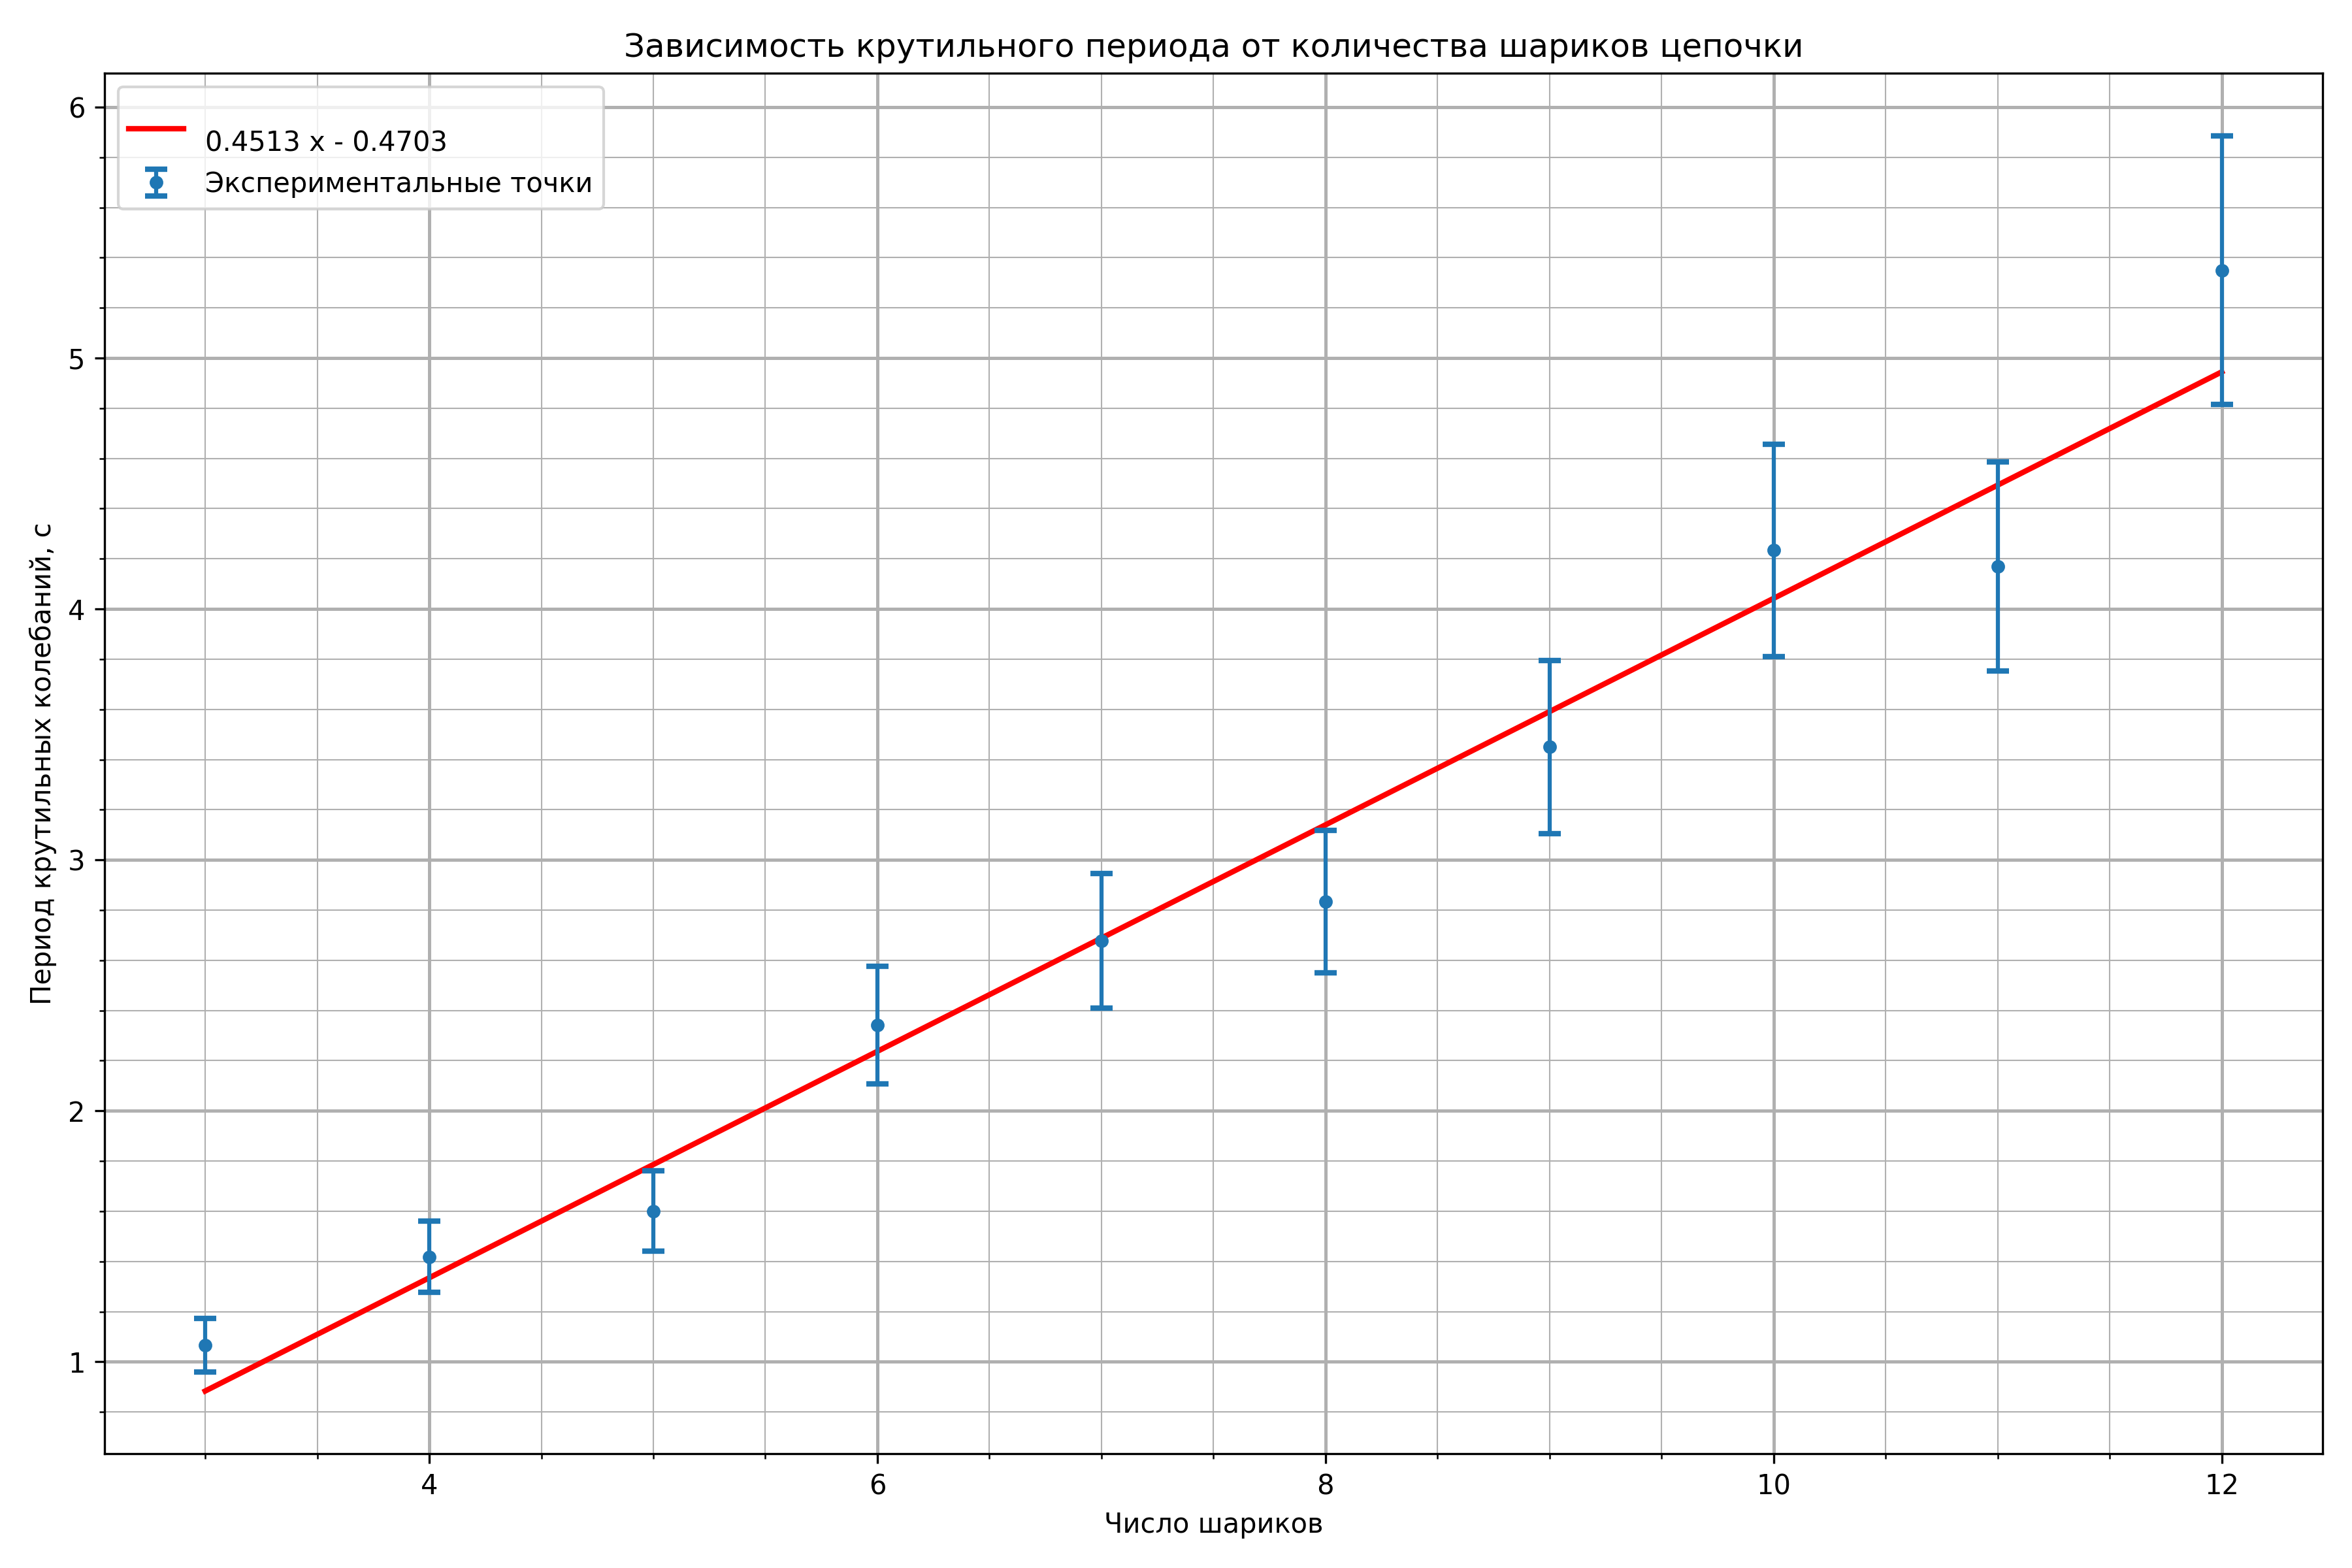
\includegraphics[width=\linewidth]{period.png}
            \caption{график крутильных колебаний стрелки}
            \label{горизонтальная составляющая}
        \end{subfigure}
        \hfill
        \begin{subfigure}{0.8\textwidth}
            \centering
            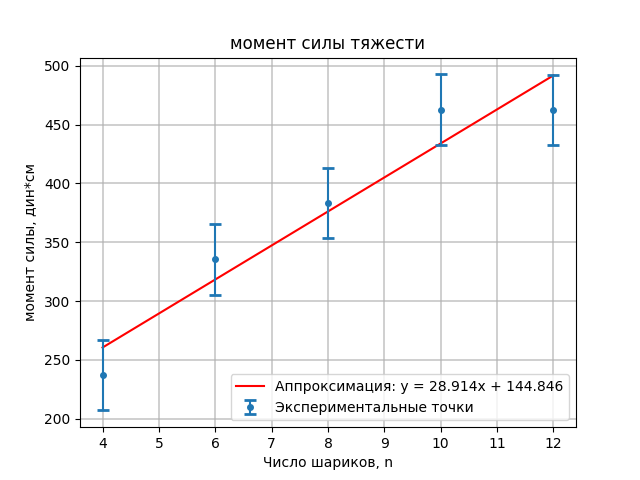
\includegraphics[width=\linewidth]{vertical.png}
            \caption{зависимость момента силы тяжести от числа шариков}
            \label{вертикальная составляющая}
        \end{subfigure}
        \caption{графики $T(n)$ и $\mathcal{M}(n)$}
        \label{графики моментов и периодов}
    \end{figure}
\end{enumerate}
\section*{Вывод}
    В работе были изучены свойства неодимовых магнитов, было измерено магнитное поле Земли, магнитное наклонение на широте Долгопрудного.
    \begin{enumerate}
        \item Неодимовые магниты хорошо подходят для изучения магнитных явлений, поскольку они обладают хорошей намагниченностью: даже самые
        маленькие кусочки обладают большой силой и магнитной энергией.
        \item Измеренное магнитное поле Земли измерение до порядка $10^{-5}$, что соответсвует порядку табличного значения.
        \item Измеренное магнитное наклонение отличается от табличного на $10^{\circ}$, это может быть связано с наличием внешнего поля,
        неточностью измерения составляющих поля.
        \item Вертикальная  составляющая больше горизонтальной, что соответсвует географическому положению Московского региона.
        \item Лабораторные установки подходят для измерения составляющих магнитного поля.
    \end{enumerate}
\end{document}
